%!TeX root = main.tex
%!encoding = UTF-8 Unicode

\chapter{Sensor and Platform Design for Methodological Implementation}

The methodology introduced in Chapter~\ref{ch:Methods} requires dedicated instrumentation to resolve the EMC-relevant, high-frequency components of the drain-source voltages and the commutation current of a switching cell for the EMC-relevant frequency range.
This chapter presents the hardware developed to realize this methodology: a dual-channel differential active voltage probe for the high-side and low-side switching-node voltages, a complementary dual-channel active current probe for the commutation current, and the measurement platform that integrates both sensors into a representative power-electronic application.

\section{Dual-Channel Differential Active Voltage Probe}
\label{ch:voltage}

Measuring the EMC-relevant high-frequency drain-source voltage components requires a probe with low noise, high bandwidth, and a short, well-defined electrical connection to the DUT terminals.
In addition, the output interface must provide a \SI{50}{\Omega} output for supplying both a low-pass and a high-pass signal path for time-domain and EMC-oriented frequency-domain evaluation, respectively.

To the best of our knowledge, no commercially available probe fully met these requirements. 
In particular, low output noise is often not a primary design target in conventional probe designs. 
Instead, many commercial probes use a large input voltage divider to keep the operational amplifier input swing small and thereby extend the bandwidth. 
However, this architecture, together with the subsequent amplification stage, can degrade the overall noise performance.



%!TeX root = main.tex
%!encoding = UTF-8 Unicode

\section{Design Constraints and Measurement Requirements}
\label{sec:VoltageRequirements}

Prior to designing the dual-channel differential active voltage probe, its requirements are established. 
These requirements are specifically tailored for discrete SiC-MOSFETs, the primary focus of this work. 
Should the target devices change to SiC power modules or GaN devices, some modifications are necessary. 
The requirements are defined in accordance with the measurement limitations introduced in section \ref{sec:MeasurementLimitation}. 

\subsubsection*{Small Signal Response}
The small signal response of the probe is characterized by its bandwidth, which must exceed the maximum frequency of interest \mi{f}{interest,max} relevant to the measurements.
As discussed in section \ref{ch:methods}, this maximum frequency differs between low-pass and high-pass measurements.
For low-pass measurements, the bandwidth requirement corresponds to the maximum frequency of voltage components still above the noise floor.
For high-pass measurements, the maximum frequency of interest is set to \SI{500}{MHz}, which represents the point at which EMC-related issues transition from being caused by semiconductor switching events to those arising from digital signal sources, such as microcontroller and FPGA clock signals.

\subsubsection*{Large Signal Response}
The large signal response of the probe is characterized by its maximum input voltage, which must exceed the maximum voltage of interest \mi{V}{interest,max} relevant to the measurements.
Since the target of this work are \SI{1200}{V} SiC-MOSFETs, the maximum voltage of interest is set to \SI{1200}{V}.
Furthermore, the minimal rise time is determined by the minimal rise time possible in a given $LC$ resonant tank.
The stray inductance of the setup is around \SI{25}{nH}, and the output capacitance of the smallest investigated MOSFET, which is a \SI{30}{A} device is \SI{74}{pF}.
The rise time of an underdamped LC resonant tank is given by:

\begin{equation}
t_r = \frac{\pi}{\omega_n\sqrt{1-\zeta^2}} - \frac{\arcsin(\zeta)}{\omega_n\sqrt{1-\zeta^2}}
\end{equation}

where the natural frequency is $\omega_n = \frac{1}{\sqrt{LC}}$ and the damping ratio is $\zeta = \frac{R}{2}\sqrt{\frac{C}{L}}$ for a series RLC circuit.

For lightly damped systems ($\zeta \ll 1$), this simplifies to:

\begin{equation}
t_r \approx 1.8\cdot\sqrt{LC}
\end{equation}

This results in a minimal rise time of approximately \SI{2.5}{ns} for the given LC parameters.
However, this value represents a purely passive response that assumes an infinitely fast switch, a condition that is typically observed only during uncontrolled diode snap-off events.
In classical operation, the switching transient is predominantly determined by the gate-drive and is typically in the range of several tens of nanoseconds.


\subsubsection*{Parasitic Coupling}
As in any practical measurement setup, parasitic coupling can occur between the probe and the DUT.
For the proposed voltage probe, the dominant mechanism is capacitive coupling from the switching-node potential into the sensitive amplification stage.
Because this influence depends strongly on layout- and setup-specific conditions, it cannot be represented by a single precise quantitative requirement.
Therefore, the final measurement results must be validated by cross-checking against a trusted reference, typically a conventional passive voltage probe.

\subsubsection*{Transmission Line Effects}
In high-frequency measurements, transmission line effects can significantly impact the accuracy of the voltage probe.
This is explicitly a problem for voltage measurement, since the source impedance of the MOSFET is changing over the switching event and the load impedance of the probe is very high in range of ${M\Omega}$.
The transmission line impedance of the connection is normally in the range of \SI{50}{\Omega} to \SI{75}{\Omega}, which is significantly lower than the input impedance of the probe.
Hence, to avoid reflections and signal distortion, the connection between the probe and the DUT must be as short as possible, but maximally

\begin{align}
    \mi{l}{max} \leq \frac{\lambda_\mathrm{min}}{10} &= \frac{c_0}{10\cdot\mi{f}{max}\sqrt{\epsilon_r}} \\
                                                    &= \frac{c_0}{10\cdot \SI{500}{MHz}\cdot \sqrt{4.25}} \\
                                                    &= \SI{2.9}{cm}
\end{align}

This allowable distance is too short to be implemented in a practically useful setup with a cable connection.
Therefore, the probe must be designed for a direct connection to the drain and source terminals of the DUT.
%!TeX root = main.tex
%!encoding = UTF-8 Unicode

\section{Probe Architecture and Implementation}
\label{sec:design_voltage}
This section presents the design of the dual-channel differential active voltage probe, which implements the methods introduced in Chapter~\ref{ch:methods} and fulfills the requirements defined in Section~\ref{sec:requirements_voltage}.

\begin{figure}[ht]
	\centering
	\import{./figures/4_VoltageProbe/}{Diss_SchematicOverviewEMEProbe.pdf_tex}
	\caption{Schematic overview of DAVP functionality.}\label{fig:OverviewEMEProbe}
\end{figure}


An overview of the probe is provided in \fref{fig:OverviewEMEProbe}, and a photograph of the implemented hardware is shown in \fref{fig:Pic_EMEProbe}.
The design is organized into three main functional blocks: the frequency-compensated voltage divider, the unity-gain stage, and the subtractor.
Each block is discussed in detail in the following, including key design considerations, encountered challenges, and the implemented solutions.

\begin{figure}[ht]
	\centering
	\import{./figures/4_VoltageProbe/}{Diss_Pic_EMEv5c.pdf_tex}
	\caption{Photograph of redesigned dual-channel differential active voltage probe.}\label{fig:Pic_EMEProbe}
\end{figure}

\subsection{Frequency-Compensated Voltage Divider}
The frequency-compensated voltage divider is the first stage of the probe and is responsible for scaling down the high-voltage signal from the DUT to a level suitable for the subsequent amplification stages.

The voltage divider is the most critical component of the probe, because of its high impedance, which creates low time constants with extremely low parasitic capacitances.
These parasitic capacitances occur due to the minimal physical distance, which are required to fulfill the requirements due to transmission line constraints, as for the necessary bandwidth constraints, which require low parasitic inductances.

The design of the frequency compensated voltage divider is shown in \fref{fig:VoltageDividerPCB_Polygon} and \fref{fig:VoltageDividerPCB}, and its equivalent schematic, including all parasitic elements, is depicted in \fref{fig:VoltageDividerPCB_parESB}.

The chosen intended parameter values are listed in \tref{tab:VoltageDividerParameters}, which design is explained in the following.

\begin{table}
	\caption{Parameter values of frequency compensated voltage divider}
	\label{tab:VoltageDividerParameters}
	\centering
	\begin{tabular}{lll}
		\toprule
		\textbf{Parameter} & \textbf{Symbol} & \textbf{Value} \\
		\midrule
		High-voltage resistor &\mi{R}{HV} & \SI{2}{M\Omega} \\
		Sense resistor &\mi{R}{sens} & \SI{2.5}{k\Omega} \\
		Sense capacitor &\mi{C}{sens} & \SI{156}{pF} \\
		High-voltage capacitor &\mi{C}{HV} & \SI{0.2}{pF} \\
		\bottomrule
	\end{tabular}
\end{table}

\begin{figure}[ht]
	\centering
	\import{./figures/4_VoltageProbe/}{Diss_VoltageDividerPCB_parESB.pdf_tex}
	\caption{Equivalent schematic of the frequency-compensated voltage divider including all parasitic elements.}\label{fig:VoltageDividerPCB_parESB}
\end{figure}

Here, the goal of a frequency compensated voltage divider is to achieve a flat frequency response over the desired bandwidth, which is accomplished by carefully selecting the resistor and capacitor values to counteract the effects of parasitic capacitances and inductances.
They need to have the same divider ratio

\begin{equation}
	\mi{a}{CR} = \frac{\mi{R}{sens}}{\mi{R}{sens} + \mi{R}{HV}} = \frac{\mi{C}{HV}}{\mi{C}{sens} + \mi{C}{HV}}.
	\label{eq:divider_ratio}
\end{equation}

The component selection is, however, constrained by the limited availability of parts suitable for both high-voltage and high-frequency applications.
The gain is designed to use the full input range of the subsequent unity-gain stage, which is \SI{2.6}{V} for a \SI{1200}{V} input signal, resulting in a divider ratio of \mi{a}{CR} = 1/460.

\subsubsection*{Sense Capacitor}
The primary bandwidth-limiting factor is the self-resonance frequency of the sense capacitor, given by
\begin{equation}
	\mi{f}{res} = \frac{1}{2\pi\sqrt{\mi{C}{sens}\cdot\mi{L}{\sigma,sens}}}.
\end{equation}
To maximize this frequency, all commercially available capacitor technologies marketed for high-frequency use were evaluated.
The measurement results for the different technologies are shown in \fref{fig:CapacitorComparison}, obtained with a VNA and measured into the high-impedance voltage divider at port 1 and the output of the unity gain stage at port 2.
This measurement setup allows for a measurement of the real behavior of the sense capcacitor without a high influence of the accuracy of the deembedding of the VNA calibration, which would be necessary with a 1-port measurement into the sense capacitor directly.
Then, the remaining error of the parasitic inductance would be included in the measurement results, which would lead to a wrong evaluation of the different capacitor technologies.

\begin{figure}[ht]
	\centering
	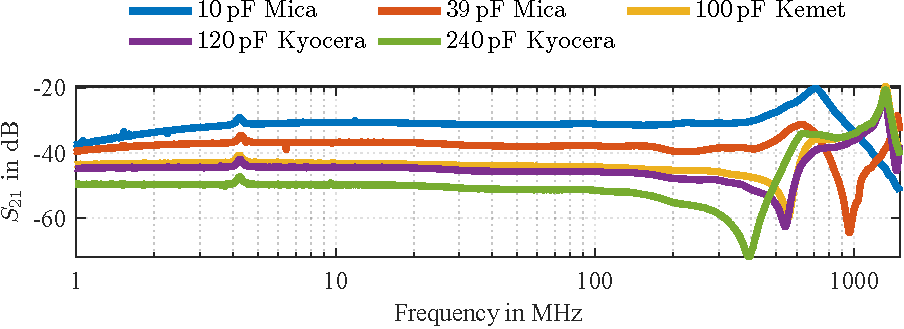
\includegraphics[scale=1]{figures/4_VoltageProbe/Voltage_Csense_Comp.pdf}
	\caption{Comparison of different sense capacitor technologies.}\label{fig:CapacitorComparison}
\end{figure}

In \fref{fig:CapacitorComparison} the different capacitance values can be seen by different amplifications of the transfer function.
Furthermore the resonance frequency can be seen, where the transfer function shows a pole, which is caused by the parasitic inductance of the sense capacitor.
This is summarized in \tref{tab:CapComp}, which shows the measured capacitance, the resonance frequency, and the calculated parasitic inductance.

\begin{table}
	\caption{Comparison of different high-frequency capacitor technologies.}
	\label{tab:CapComp}
	\centering
	\begin{tabular}{l l l l l}
		\toprule
		Manufacturer & Technology & Capacitance & Resonance Frequency & Calc. Inductance\\
		\midrule
		{Illinois} {Capacitor} & Mica & \SI{10}{pF} & -- & -- \\
		{Illinois} {Capacitor} & Mica & \SI{39}{pF} & \SI{956}{MHz} & \SI{710}{pH} \\
		Kemet & MLCC & \SI{100}{pF} & \SI{555}{MHz} & \SI{822}{pH} \\
		Kyocera & MLCC & \SI{120}{pF} & \SI{540}{MHz} & \SI{723}{pH} \\
		Kyocera & MLCC & \SI{240}{pF} & \SI{393}{MHz} & \SI{683}{pH} \\
		\bottomrule
	\end{tabular}
\end{table}

All technologies show a similar parasitic inductance, which is in the range of \SI{700}{pH} to \SI{800}{pH}.
This leads to the explanation, that not the used technology defines the parasitic inductance, but the package size of it, which is the same for all them: a standard 0805 package.

The goal is to achieve a maxmimum sense capacitance, while keeping the resonance pole well above \SI{500}{MHz}, which is the targeted bandwidth of the probe.

A classical approach to increase the capacitance, without decreasing resonance frequency, is to connect multiple capacitors in parallel, which is done for the \SI{39}{pF} mica capacitor shown in \fref{fig:CsenseParallel}.
Here, the expectation is, that the resonance capacitance value is increased by the number of parallel capacitors, while the parasitic inductance is decreased by the same factor, hence, resulting in a constant resonance frequency.
However, the measurement results show, that the resonance frequency is decreasing for an increasing number of capacitors, which is caused by remaining parasitic inductance of the PCB between parallel-connected capacitors.

\begin{figure}[ht]
	\centering
	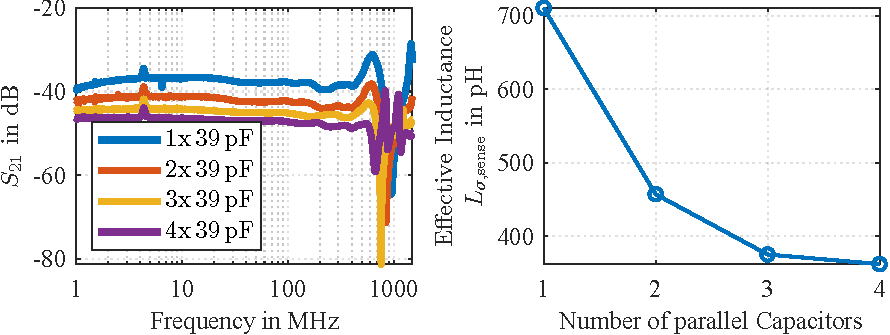
\includegraphics[scale=1]{figures/4_VoltageProbe/Voltage_Csense_parallel.pdf}
	\caption{Behavior of parallel-connected sense mica capacitors.}\label{fig:CsenseParallel}
\end{figure}

As can be seen, a maximum number of four capacitors can be connected in parallel, which results in a total capacitance of \SI{156}{pF} and a resonance frequency of \SI{670}{MHz}, which is the targeted bandwidth of the probe.
In \fref{fig:CsenseParallel} also the calculated parasitic inductance is plotted; for a number of four parallel capacitors, the parasitic inductance has only reduced by a factor of 1.9.




\subsubsection*{High-Voltage Capacitor \mi{C}{HV}}
After the selection of the sense capacitor, the high-voltage capacitor \mi{C}{HV} is designed to achieve the desired divider ratio of \eref{eq:divider_ratio}.
Here, the high-voltage capacitor is the remaining part of the high-voltage capacitance, which is necessary to achieve the desired divider ratio, which is not created by the parasitic capacitance \mi{C}{\sigma 1,HV} of the high-voltage resistor \mi{R}{HV}, see \fref{fig:VoltageDividerPCB_parESB}.

\begin{figure}[ht]
	\centering
	\import{./figures/4_VoltageProbe/}{Diss_VoltageDividerPCB_Querschnitt.pdf_tex}
	\caption{Cross-section of the redesigned dual-channel differential active voltage probe PCB.}\label{fig:VoltageDividerPCB}
\end{figure}

It can be calculated as:
\begin{equation}
	\mi{C}{HV} = \frac{\mi{C}{sens}}{\mi{a}{CR}} - \mi{C}{\sigma 1,HV}.
\end{equation}
Given the lack of high-voltage, high-frequency capacitor technologies, a custom PCB-integrated parallel-plate capacitor was implemented. 
The capacitor is realized symmetrically: the positive signal path employs the copper layers between the top and second PCB layer, while the negative signal path utilizes the corresponding layers between the bottom and fifth PCB layer. 
This symmetric implementation ensures balanced performance across both differential channels.
Its capacitance can be calculated using the classical parallel-plate capacitor formula: cite
\begin{equation}
	\mi{C}{HV} = \frac{\varepsilon_0 \cdot \varepsilon_r \cdot A}{d},
\end{equation}
Since, both the parasitic capacitance \mi{C}{\sigma 1,HV} of the high-voltage resistor as the width of the prepreg of the PCB have significant tolerances, the effective electrode area of the PCB capacitor is designed to be trimmable by adjusting the overlap of the top and bottom copper layers.
This is realized by the finger layout of the polygon, which can be seen in \fref{fig:VoltageDividerPCB_Polygon}.

\begin{figure}[ht]
	\centering
	\import{./figures/4_VoltageProbe/}{Diss_VoltageDividerPCB_Polygons.pdf_tex}
	\caption{Finger layout of the trimmable PCB capacitor.}\label{fig:VoltageDividerPCB_Polygon}
\end{figure}

\subsubsection*{High-Voltage Resistor \mi{R}{HV} and Sense Resistor \mi{R}{sens}}
The resistor choice is has only secondary interests for this work, since the main focus of thsi work is the high frequncy behavior of the probe, which is mainly defined by the capacitive elements of the voltage divider.
The cut-off frequency of the voltage divider is defined by the RC time constant of the high-voltage resistor \mi{R}{HV} and the sense capacitor \mi{C}{sens}, which is given by cite
\begin{align}	
	\mi{f}{c} &= \frac{1}{2\pi \cdot \mi{R}{HV} \cdot \mi{C}{HV}} \\
				&= \frac{1}{2\pi \cdot \SI{2}{M\Omega} \cdot \SI{0.2}{pF}} = \SI{500}{kHz}	
\end{align}

For the high-voltage resistor \mi{R}{HV}, a rather low resiatnce value was chosen in contrast to commercially available high-voltage probes, which typically use a \SI{10}{M\Omega} resistor.
This is done due to problems with the parasitic capacitance \mi{C}{\sigma 2,HV} of the high-voltage resistor, which is causes time constants in the relevant frequency regime.
This was reduced, by choosing a smaller resistor value, changing the resistor technology from a thick-film resistor to a thin-film resistor, and by creating a PCB cutout region just below the resistor, see \fref{fig:VoltageDividerPCB_Polygon}.

\subsubsection*{Shielding}
In a previous version the probe consists of a four-layer PCB, which caused a crosscoupling from the positive to the negative side and vice versa through the parasitic capacitance \mi{C}{\sigma 2,sens}.
This can be reduced by adding an additional shielding layer between the positive and negative signal path, which is implemented in a six-layer PCB, see \fref{fig:VoltageDividerPCB}.













\subsection{Unity Gain Amplifier}
The output of voltage divider is a signal of changing impedance over frequency contributed to the sense capacitance.
To gain a constant output impedance over frequency, a unity-gain stage is implemented.
This unity gain amplifier requires a low-noise, high-bandwidth, and high-input impedance amplifier to avoid loading the voltage divider and to maintain signal integrity.
Furthermore, for classical analysis like overshoot, \sddt{v} and \mi{e}{sw} an accurate DC measurement is required.



A composite loop amplifier architecture was selected for the probe's unity gain buffer to achieve both high DC precision and a wide bandwidth, a combination that is challenging to attain with a single amplifier. 
Precision operational amplifiers offer excellent DC accuracy (low offset and drift) but have limited gain-bandwidth products. 
Conversely, high-speed buffers provide multi-gigahertz bandwidth and high slew rates but typically have poorer DC characteristics. 
The composite loop topology leverages the strengths of two different amplifiers by creating separate signal paths for low-frequency and high-frequency signal components, which are then seamlessly recombined at the output.
The chosen composite loop amplifier architecture is depicted in \fref{fig:EME_ESB_UG}, where the low-frequency path is handled by a precision operational amplifier, while the high-frequency path is managed by a high-speed buffer.

\begin{figure}[ht]
	\centering
	\import{./figures/4_VoltageProbe/}{Diss_UnityGain_EME_ESB.pdf_tex}
	\caption{Equivalent circuit diagram of the unity-gain stage, which is designed as a composite loop amplifier.}\label{fig:EME_ESB_UG}
\end{figure}

\begin{table}[ht]
	\caption{Parameter values of Unity Gain Amplifier}
	\centering
	\begin{tabular}[t]{l l}
		\toprule
		\textbf{Parameter} & \textbf{Value}\\
		\midrule
		\mti{OP}{1} & BUF802 			\\
		\mi{R}{1} & \SI{52.2}{k\Omega}	\\
		\mi{R}{3} & \SI{30}{\Omega}		\\		
		\mi{R}{5} & \SI{10}{k\Omega}	\\
		\mi{R}{8} & \SI{10}{\Omega}		\\
		\mi{C}{1} & n.p. 				\\
		\mi{C}{3} & \SI{27}{pF}			\\
		\bottomrule
	\end{tabular}
	\hspace{1cm}
	\begin{tabular}[t]{l l}
		\toprule
		\textbf{Parameter} & \textbf{Value}\\
		\midrule
		\mti{OP}{2} & OPA140 \\
		\mi{R}{2} & \SI{11}{k\Omega} \\
		\mi{R}{4} & \SI{2.44}{k\Omega} \\
		\mi{R}{6} & \SI{2}{k\Omega} \\
		\mi{R}{9} & \SI{80}{k\Omega}\\
		\mi{C}{2}  & \SI{270}{pF} \\
		\mi{C}{4} & \SI{100}{pF} \\
		\bottomrule
	\end{tabular}
\end{table}

The input signal is split into two paths using a frequency-dependent network.
A series capacitor \mi{C}{2} and a resistor \mi{R}{3} on the input of the high frequency OP \mti{OP}{1} form a high-pass filter. 
This directs high-frequency signals to the fast buffer path with the open loop gain $G$. 
The precision amplifier \mti{OP}{2} handles the signal for the auxiliary path, which dominates the low-frequency response. 

To ensure a flat frequency response across the crossover region where both amplifiers are active, the gain of the low-frequency path must precisely match the gain of the high-frequency path. 
The datasheet specifies the condition 
\begin{align}
	\sfrac{\alpha}{\beta} &= G \\
	\alpha &= \frac{\mi{R}{2}}{\mi{R}{1} + \mi{R}{2}}  \\
	\beta &= \frac{\mi{R}{4}}{\mi{R}{4} + \mi{R}{5}}
\end{align}

where $\alpha$ is the input attenuation factor of the precision amplifier path, and $\beta$ is the feedback factor of the precision amplifier.
Since the gain $G$ can vary between devices, the precision amplifier's feedback network must be trimmed during commissioning.

Lastly, same gain must be achieved for the positive and negative unity gain amplifier.
This is different from device to device and additionally changed due to the different load of the two unity gains due to the asymmetrical load of the subtractor, which is connected to the output of the unity gain amplifier.
To still achieve the same gain for both unity gain amplifiers, a voltage divider by \mi{R}{8} and \mi{R}{9} is implemented, which must be trimmed during comissioning.
Any asymmetry in the gain of the unity gain amplifiers would lead to a non-zero output of the subtractor, which directly worsens the CMRR.


\begin{figure}[ht]
	\centering
	\input{"figures/4_VoltageProbe/VNA_rawUG.tex"}
	\caption{VNA measurement of unity gain amplifier.}\label{fig:VNA_rawUG}
\end{figure}

\subsection{Dual-Channel Subtractor}
Up to this point, the probe design is similar to conventional differential probes, which typically employ a single subtractor stage to generate the differential output signal.
However, now the signal is split into two separate paths, each with its own dedicated subtractor stage.
The low-pass - or conventional - subtractor amplifier is designed to provide a flat frequency response up to the frequency, where the signal falls below the noise floor (normally around \SI{120}{MHz})).
The high-pass subtractor amplifier is designed to provide a frequency response of \SI{+40}{dB/dec} to enable an analysis of the EMC-relevant frequency range, as discussed in Chapter \ref{ch:Methods}.

\subsubsection*{Low-Pass Subtractor}
The equivalent circuit diagram of the low-pass subtractor is shown in \fref{fig:EME_ESB_LP} and its used parameter values in \tref{tab:ComponentsLowPass_Voltage}.

\begin{figure}[ht]
	\centering
	\import{./figures/4_VoltageProbe/}{Diss_Lowpass_EME_ESB.pdf_tex}
	\caption{Equivalent circuit diagram of the low-pass subtractor.}\label{fig:EME_ESB_LP}
\end{figure}

\begin{table}[ht]
	\caption{Parameter values of the low-pass subtractor.}
	\label{tab:ComponentsLowPass_Voltage}
	\centering
	\begin{tabular}[t]{l l}
		\toprule
		\textbf{Parameter} & \textbf{Value}\\
		\midrule
		\mti{OP}{LP} & OPA817 		\\
		\mi{R}{10} & \SI{180}{\Omega}\\
		\mi{R}{11} & \SI{180}{\Omega}\\		
		\mi{R}{12} & \SI{180}{\Omega}\\
		\bottomrule
	\end{tabular}
	\hspace{1cm}
	\begin{tabular}[t]{l l}
		\toprule
		\textbf{Parameter} & \textbf{Value}\\
		\midrule
		\mi{R}{13} & \SI{180}{\Omega}\\
		\mi{R}{14} & \SI{10}{\Omega} \\
		\mi{C}{5} & n.p.			 \\
		\mi{C}{6} & n.p.			 \\
		\bottomrule
	\end{tabular}
\end{table}

The circuit follows a classical differential amplifier topology, where the output voltage is given by
\begin{equation}
	\mi{v}{LP} = \mi{v}{UG+}\cdot\frac{\mi{R}{11}}{\mi{R}{10}+\mi{R}{11}}\left(\frac{\mi{R}{12}}{\mi{R}{12}+\mi{R}{13}}\right) - \mi{v}{UG-}\cdot\frac{\mi{R}{13}}{\mi{R}{12}} \\
\end{equation}
which simplifies for a symmetric design of the resistors $\mi{R}{10} = \mi{R}{12}$ and $\mi{R}{11} = \mi{R}{13}$
\begin{equation}
	\mi{v}{LP} = \frac{\mi{R}{11}}{\mi{R}{10}} \cdot (\mi{v}{UG+} - \mi{v}{UG-})
\end{equation}

If a defined cut-off frequency is desired, the output can be low-pass filtered by adding capacitors \mi{C}{5} and \mi{C}{6} in parallel to the feedback resistors \mi{R}{13} and \mi{R}{14}, respectively.
However, in the current design, these capacitors are not populated, and the roll-off is defined by the operational amplifier.

\begin{figure}[ht]
	\centering
	\input{"figures/4_VoltageProbe/VNA_rawLP.tex"}
	\caption{VNA measurement of low-pass substractor.}\label{fig:VNA_rawLP}
\end{figure}

\subsubsection*{High-Pass Subtractor}
The high-pass subtractor is designed to provide a frequency response of \SI{+40}{dB/dec} to enable an analysis of the EMC-relevant frequency range, as discussed in Chapter \ref{ch:Methods}.
The equivalent circuit diagram of the high-pass subtractor is shown in \fref{fig:EME_ESB_HP} and its used parameter values in \tref{tab:ComponentsHighPass_Voltage}.

\begin{figure}[ht]
	\centering
	\import{./figures/4_VoltageProbe/}{Diss_Highpass_EME_ESB.pdf_tex}
	\caption{Equivalent circuit diagram of the high-pass filter.}\label{fig:EME_ESB_HP}
\end{figure}

\begin{table}[ht]
	\caption{Parameter values of the high-pass subtractor.}
	\label{tab:ComponentsHighPass_Voltage}
	\centering
	\begin{tabular}[t]{l l}
		\toprule
		\textbf{Parameter} & \textbf{Value}\\
		\midrule
		\mti{OP}{HP1} & LMH5401 		\\
		\mi{C}{7}, \mi{C}{8} & \SI{6}{pF}\\
		\mi{R}{15}, \mi{R}{16} & \SI{10}{\Omega}\\
		\mi{R}{17}, \mi{R}{18} & \SI{400}{\Omega}\\	
		\mi{R}{fb} & \SI{25}{\Omega}\\
		\mi{R}{out} & \SI{10}{\Omega}\\
		\mi{R}{19},\mi{R}{20} & \SI{10}{\Omega}\\
		\bottomrule
	\end{tabular}
	\hspace{0.5cm}
	\begin{tabular}[t]{l l}
		\toprule
		\textbf{Parameter} & \textbf{Value}\\
		\midrule
		\mti{OP}{HP2} & LMH5401 		\\
		\mi{C}{9}, \mi{C}{10} & \SI{6}{pF}\\
		\mi{R}{21}, \mi{R}{22} & \SI{10}{\Omega}\\		
		\mi{R}{23}, \mi{R}{24} & \SI{200}{\Omega}\\		
		\mi{R}{fb} & \SI{25}{\Omega}\\
		\mi{R}{out} & \SI{10}{\Omega}\\
		\mi{R}{25}, \mi{R}{26} & \SI{10}{\Omega}\\
		\bottomrule
	\end{tabular}
	\hspace{0.5cm}
	\begin{tabular}[t]{l l}
		\toprule
		\textbf{Parameter} & \textbf{Value}\\
		\midrule
		\mti{OP}{HP3} & THS4302\\
		\mi{R}{27} & \SI{50}{\Omega}\\		
		\mi{R}{28} & \SI{200}{\Omega}\\
		\mi{R}{g} & \SI{50}{\Omega}\\		
		\mi{R}{f} & \SI{200}{\Omega}\\	
		\mi{R}{29} & \SI{10}{\Omega}\\
		\bottomrule
	\end{tabular}
\end{table}

The high-pass subtractor uses a cascaded design.
The gain can be calculated as
\begin{equation}
	\mi{v}{HP} = \mi{G}{HP1} \cdot \mi{G}{HP2} \cdot \mi{G}{HP3} \cdot (\mi{v}{UG+} - \mi{v}{UG-})
\end{equation}
with
\begin{align}
	\mi{G}{HP1} &= \frac{s\omega \mi{C}{7}(\mi{R}{17}+ \mi{R}{fb})}{s\omega \mi{C}{7}\mi{R}{15}+1}\\
	\mi{G}{HP2} &= \frac{s\omega \mi{C}{9}(\mi{R}{23}+ \mi{R}{fb})}{s\omega \mi{C}{9}\mi{R}{21}+1}\\
	\mi{G}{HP3} &= \frac{\mi{R}{f}}{\mi{R}{g}}
\end{align}

again, for total symmetry between positive and negative signal path, the same component values are used for both channels.
	

Although a second-order high-pass response could in principle be realized with a single stage, this would result in increased signal attenuation due to the additional high-pass impedance.
Since the voltage divider already introduces a large attenuation, compensating gain is required to raise the signal to a level suitable for the oscilloscope input while keeping it well above the oscilloscope's noise floor.
This represents a careful design trade-off: increasing the gain of the secondary amplifier stage also amplifies its noise contribution, potentially degrading the overall signal-to-noise ratio.
Following Friis' noise formula for cascaded systems, the noise figure of the chain is governed by
\begin{equation}
	\mi{F}{total} = \mi{F}{1} + \frac{\mi{F}{2}-1}{\mi{G}{1}} + \frac{\mi{F}{3}-1}{\mi{G}{1}\cdot\mi{G}{2}} + \cdots
\end{equation}
which shows that the first stage dominates the overall noise performance.
Consequently, the first stage carries the highest gain, while the second stage contributes only the additional filter order required to achieve the desired \SI{+40}{dB/dec} slope.
The final stage converts the differential signal to a single-ended output; using only one of the two differential outputs was also evaluated but resulted in a lower SNR.


\begin{figure}[ht]
	\centering
	\input{"figures/4_VoltageProbe/VNA_rawHP.tex"}
	\caption{VNA measurement of high-pass substractor. (xxx must be repeated)}\label{fig:VNA_rawHP}
\end{figure}

Figure~\ref{fig:VNA_rawHP} shows the measured frequency response of the high-pass subtractor, which confirms the expected \SI{+40}{dB/dec} slope up to the cutoff-frequency of the high-pass at \SI{400}{MHz}.
At the the cutoff frequency, the final gain is \SI{27}{dB}.

\subsection{Shielding Concept and Implementation}

Last part of the probe for a full functional design is the shielding concept, which is necessary to avoid parasitic couplings from the environment to the probe and vice versa.
Here, the main noise source is the switching node potential, which is in close proximity to the probe and, hence, is susceptible to capacitive couplings.

Therefore, the probe is shielded by a metal housing, which is connected to the analog ground potential and thereby, the oscilloscope ground.
A photograph of the housing is depicted in \fref{fig:Pic_EMEProbe}.
The high-voltage and active amplification circuitries are shielded separately, however to avoid ground loops, they are manufactured as a single aluminum block, which is milled to create the necessary cavities for the functional blocks.


xxx add measurement with and without shielding.


%!TeX root = main.tex
%!encoding = UTF-8 Unicode

\section{Verification}
This section provides a rigorous verification of the dual-channel differential active voltage probe.
This probe enables access to high-frequency drain-source voltage components that are not reliably captured by conventional probe solutions; therefore, verification is treated as a central requirement rather than a supplementary step.
Accordingly, a comprehensive set of verification measurements is conducted to demonstrate that the relevant error mechanisms introduced in Section~\ref{sec:fundamental_measurement_errors} do not materially distort the reported results.

The updated probe was validated using the methodology of~\cite{kragl_active_2025}: small-signal characterization with a vector network analyzer (VNA), large-signal verification with a \SI{50}{\ohm} pulse generator, and low-pass cross-verification against a standard passive probe to exclude unintended capacitive or inductive coupling into the active measurement path.









\subsection{Small-Signal Verification for Differential Probes}
The first test is a small-signal verification using a VNA to measure the frequency response of both the low-pass and high-pass channels.
The VNA was calibrated using an Open-Short-Load procedure at the probe input, with the VNA source impedance set to \SI{50}{\Omega}.
Measurements focus on the magnitude response to validate gain flatness for the low-pass channel and to verify bandwidth performance for both channels.

Since the probe is designed for differential operation but only a two-port VNA is available, the measurement is conducted in two separate single-ended configurations, as illustrated in \fref{fig:EME_VNA_SchematicOverview}.
The shared ground potential of the two VNA ports effectively shorts the differential input not under test, so only one input path can be characterized at a time.
The measurement is therefore repeated with the positive and negative differential inputs swapped, yielding the frequency response for both signal paths individually.
Comparing the two results also reveals the degree of input symmetry, which is directly relevant to the probe's common-mode rejection ratio (CMRR).

\begin{figure}[ht]
	\centering
	\import{./figures/4_VoltageProbe/}{Diss_SchematicOverview_EME_VNA.pdf_tex}
	\caption{Small-signal verification setup: single-ended VNA measurement of one differential input at a time. The VNA ground connection shorts the inactive differential input; the measurement is repeated with swapped connections to characterize both input paths.}\label{fig:EME_VNA_SchematicOverview}
\end{figure}

The design targets are a bandwidth exceeding \SI{120}{MHz} for the low-pass channel (where the noise floor typically emerges in power electronics measurements) and \SI{500}{MHz} for the high-pass channel.

The VNA results for the low-pass and high-pass channels are shown in \fref{fig:VNA_LP} and \fref{fig:VNA_HP}, respectively.
Here both differential inputs are measured, where the positive signal path is plotted with a solid line and the negative signal path with a dashed line.
Additionally, the measurement was executed with \SI{0}{dBm} input power for the positive and \SI{-10}{dBm} for the negative input.
This can be seen in the corresponding different noise floors at \SI{-100}{dB} and \SI{-80}{dB} for the positive and negative input of \mti{S}{11,LP}, respectively.

\begin{figure}[ht]
	\centering
	\input{"figures/4_VoltageProbe/VNA_LP.tex"}
	\caption{VNA measurement of positive (LPp) and negative (LPn) low-pass paths, crosscheck~\fref{fig:EME_VNA_SchematicOverview}.}\label{fig:VNA_LP}
\end{figure}

From this measurement also the probe voltage gain \mti{a}{probe} is obtained from the S-parameter measurement as
\begin{align}
	\mti{a}{probe} 	&= \frac{\mi{v}{out}}{\mi{v}{HV+}-\mi{v}{HV-}} \\
					&= \frac{\mti{S}{21}}{1 + \mti{S}{11}}.
\label{eq:TF_probe}
\end{align}

Since \mti{S}{11} remains nearly constant because of the probe's high input impedance, \mti{S}{21} is the dominant parameter for gain evaluation.
This expression holds under the assumption of equal gain in both differential input paths, a condition verified by the symmetry measurements described above.
In the presence of a gain mismatch, the effective transfer function would depend on the common-mode voltage partitioning between the two inputs — determined by the oscilloscope ground potential relative to the drain-source midpoint — a quantity that is generally undefined during in-circuit measurements.

The low-pass channel exhibits a flat passband gain of \SI{-53}{dB}, corresponding to a voltage division ratio of 446, in close agreement with the voltage divider design value.
The gain remains flat across the passband and rolls off at a \SI{3}{dB} bandwidth of \SI{315}{MHz}, primarily limited by the low-pass subtractor operational amplifier (see \fref{fig:VNA_rawLP}).
This substantially exceeds the design target of \SI{120}{MHz}, providing ample margin across the frequency range relevant to power electronics measurements.
The two input paths show close gain agreement, with a maximum deviation of \SI{0.2}{dB} at \SI{3}{MHz}, confirming the high degree of symmetry required for accurate differential measurements.

The high-pass channel, shown in \fref{fig:VNA_HP}, exhibits a gain slope of approximately \SI{+40}{dB/dec} from \SI{1}{MHz} to \SI{450}{MHz}, beyond which the unity-gain output amplifier begins to roll off.
The input-path gain deviation remains below \SI{0.8}{dB} within the linear-gain region, but increases to \SI{2.8}{dB} at \SI{490}{MHz} as both paths approach their respective rolloff frequencies.
The \SI{3}{dB} bandwidth exceeds the \SI{400}{MHz} lower design target, confirming that the channel adequately resolves high-frequency switching harmonics.
For measurements extending to \SI{500}{MHz}, the growing input-path gain mismatch must be considered, as it introduces an increasing common-mode error in the differential result.

\begin{figure}[ht]
	\centering
	\input{"figures/4_VoltageProbe/VNA_HP.tex"}
	\caption{VNA measurement of positive (HPp) and negative (HPn) high-pass paths, crosscheck~\fref{fig:EME_VNA_SchematicOverview}.}\label{fig:VNA_HP}
\end{figure}

In both measurements, a pole of the voltage divider is apparent at \SI{695}{MHz}, attributed to the RC network that establishes the probe input impedance.

\mti{S}{22} confirms the \SI{10}{\Omega} output resistance in both channels, consistent with the design specification for use with appropriate attenuators in \SI{50}{\Omega} measurement systems.
\mti{S}{11} reflects the high-impedance input of the voltage divider, yielding an approximately \SI{0}{dB} reflection coefficient and confirming negligible loading on the circuit under test.
\mti{S}{12} reveals a residual passive coupling path from output to input; however, this reverse transmission remains sufficiently small that it does not materially affect measurement accuracy within the verified frequency range.













\subsection{Large-Signal Verification with High-Voltage \SI{50}{\Omega} Pulse Generator}
In addition to the small-signal VNA characterization, the probe was validated by a large-signal measurement using a \SI{400}{V}, \SI{50}{\ohm} pulse generator.
The schematic of the measurement setup is shown in \fref{fig:MS_PulsGen_SchematicOverview}.

\begin{figure}[ht]
	\centering
	\import{./figures/4_VoltageProbe/}{Diss_PulseGenerator_ESB.pdf_tex}
	\caption{Large-signal verification of the low-pass and high-pass channels using a \SI{50}{\ohm} pulse generator~\cite{kragl_active_2025}. The reference is acquired both via a conventional direct measurement and through a commercial \SI{180}{MHz}--\SI{340}{MHz} passive band-pass filter.}\label{fig:MS_PulsGen_ESB}
\end{figure}

This setup provides a well-characterized reference voltage signal attenuated by \SI{40}{dB} through a \SI{50}{\Omega} resistor, enabling direct connection to the oscilloscope without additional impedance mismatch.
The measurement system bandwidth is determined by the oscilloscope (\SI{2}{GHz}), which is sufficient to resolve transients in the millisecond to sub-microsecond range.
A photograph of the measurement setup is shown in \fref{fig:MS_PulsGen_Pic}.

\begin{figure}[ht]
	\centering
	\import{./figures/4_VoltageProbe/}{Diss_PulseGenerator_Pic.pdf_tex}
	\caption{Large-signal verification of the low-pass and high-pass channels using a \SI{50}{\ohm} pulse generator~\cite{kragl_active_2025}. The reference is acquired both via a conventional direct measurement and through a commercial \SI{180}{MHz}--\SI{340}{MHz} passive band-pass filter.}\label{fig:MS_PulsGen_Pic}
\end{figure}

The pulse generator employs \SI{750}{V} GaN-HEMTs with the \SI{40}{dB} attenuator serving as the load, producing fast resistive switching transients with risetimes below \SI{10}{ns}.
This transient speed is critical for validating the probe's ability to capture high-frequency switching dynamics without significant slew-rate-induced errors.
The \SI{50}{\Omega} output impedance of the pulse generator also enables direct connection of commercial BNC band-pass filters, allowing independent verification of different frequency bands without the noise-limiting effects of broadband low-pass filtering.


\fref{fig:MS_PulsGen_TD} presents the time-domain measurement of the low-pass channel, comparing three signals: the attenuated pulse generator reference, a commercial passive high-voltage probe, and the DAVP low-pass channel.
The low-pass channel bandwidth (\SI{315}{MHz} from VNA measurements) is sufficient to capture the primary switching transient; however, a second-order transient response emerges during the tail, attributed to slew-rate limiting of the low-pass subtractor operational amplifier at signal levels exceeding \SI{2}{Vpp}.
The small-signal bandwidth of this op-amp (\SI{800}{MHz} at \SI{100}{mVpp}) degrades to \SI{250}{MHz} at \SI{2}{Vpp} and \SI{140}{MHz} at \SI{4}{Vpp} according to the datasheet.
In contrast, the shared unity-gain buffer amplifier (used by both channels) exhibits minimal slew-rate effects, with measured bandwidths of \SI{3.1}{GHz} at \SI{100}{mVpp} and \SI{1.6}{GHz} at \SI{2}{Vpp}.
The DAVP low-pass channel accurately captures the initial rising edge of the transient.
However, the PT2 behavior present in the transient tail introduces a waveform distortion that results in a settling time of around \SI{20}{ns} before the final value is reached.
Since this effect is confined to the low-pass subtractor amplifier, it does not affect the high-pass channel.


\begin{figure}[ht]
	\centering
	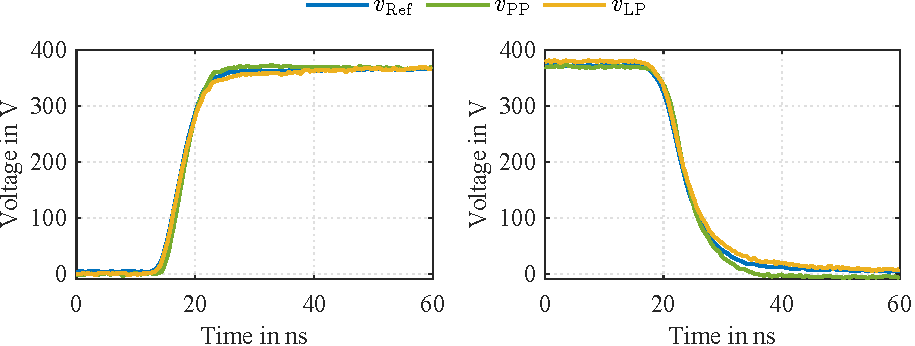
\includegraphics[scale=1]{figures/4_VoltageProbe/MS_PulsGen_TD.pdf}
	\caption{Large-signal verification time-domain of the low-pass using a \SI{50}{\ohm} pulse generator~\cite{kragl_active_2025}. The reference is acquired both via a conventional direct measurement and through a commercial \SI{180}{MHz}--\SI{340}{MHz} passive band-pass filter.}\label{fig:MS_PulsGen_TD}
\end{figure}

For high-pass channel verification, the pulse generator output is passed through a commercial \SI{180}{MHz}--\SI{340}{MHz} passive BNC band-pass filter, which isolates the high-frequency components while attenuating the DC and low-frequency content.
For this verification it is only useful to compare the calibrated frequency domain results, because the band-pass and the high-pass channel have completely different time-domain responses.
The frequency-domain results are shown in \fref{fig:MS_PulsGen_Meas}, comparing four traces: the unfiltered reference spectrum, the band-pass filtered reference spectrum, the low-pass channel spectrum, and the high-pass channel spectrum.
A sequence of pulses ensures matched quantization noise floors between the reference and measurement channels, enabling direct amplitude comparison.

\begin{figure}[ht]
	\centering
	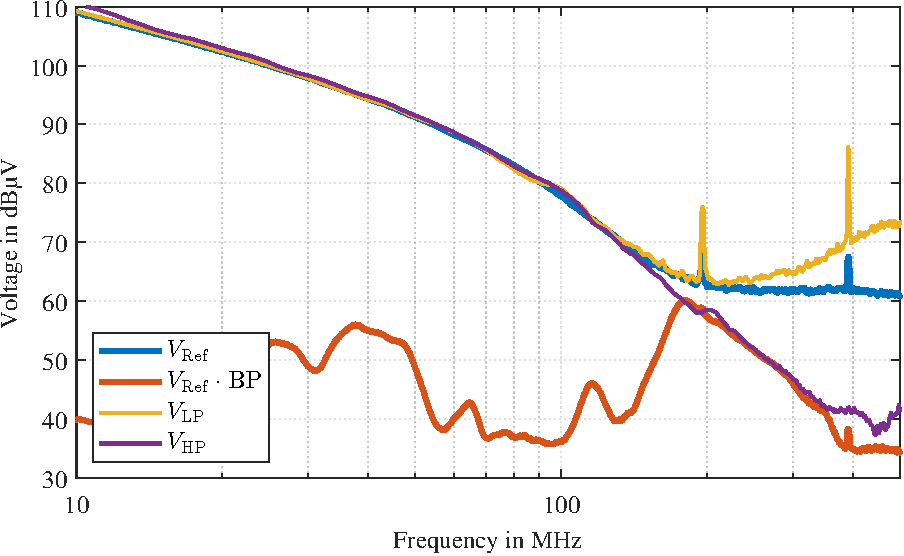
\includegraphics[scale=1]{figures/4_VoltageProbe/MS_PulsGen.pdf}
	\caption{Large-signal verification of the low-pass and high-pass channels using a \SI{50}{\ohm} pulse generator~\cite{kragl_active_2025}. The reference is acquired both via a conventional direct measurement and through a commercial \SI{180}{MHz}--\SI{340}{MHz} passive band-pass filter.}\label{fig:MS_PulsGen_Meas}
\end{figure}

At frequencies where the reference remains above the noise floor, the high-pass channel shows close agreement with both the reference and the low-pass channel, with a gradually increasing deviation below \SI{10}{MHz} as the high-pass channel attenuates the low-frequency content by design.
Within the band-pass filter passband (\SIrange{180}{340}{MHz}), the high-pass channel exhibits a maximum deviation of \SI{1.3}{dB} at \SI{200}{MHz}, with deviations below \SI{1}{dB} across most of the band.
Above \SI{340}{MHz}, independent verification is no longer possible, as no commercially available band-pass filter covers the \SIrange{300}{400}{MHz} region.
In this unverified range, the measured spectrum exhibits a plateau rather than the expected continuous rolloff, indicating a measurement artifact that may increase the error beyond \SI{1.3}{dB}.
Accordingly, results presented in the following analysis are shown up to \SI{500}{MHz}, but the probe is fully verified only up to \SI{340}{MHz}; results above this frequency should be interpreted as comparative rather than absolute calibrated values.


In summary, both channels satisfy their respective large-signal verification objectives.
The low-pass channel reliably captures the initial switching edge despite the slew-rate-induced PT2 behavior in the transient tail.
The high-pass channel demonstrates a maximum deviation of \SI{1.3}{dB} across the verified frequency range, consistent with the small-signal characterization results.
Together, these results confirm that the DAVP performs as designed under large-signal conditions relevant to power semiconductor measurements.











\subsection{Parasitic Couplings \& CM error}

In a next verification step, the probe is assessed in the intended application environment by measuring the drain-source voltage of a SiC MOSFET during switching transients with both a commercial passive probe and the proposed DAVP.
The setup corresponds to the commutation cell used later in this work, operated in double-pulse mode with the actively switched device located in the low-side position.

The purpose of this measurement is twofold: first, to exclude unintended parasitic coupling paths introduced by the active probe; and second, to quantify the residual common-mode error under realistic switching conditions.
Both effects could distort the measured drain-source voltage and would therefore directly limit the interpretability of the later application measurements.
Because the passive reference probe is subject to the same quantization-noise limitations as all conventional measurements in the high-frequency region, the comparison is primarily performed in the time domain.
The corresponding results are shown in \fref{fig:Voltage_DPT_LPvsPP_weCM_TD} and \fref{fig:Voltage_DPT_HPvsPP_weCM_TD}.
For the dedicated common-mode measurement, both differential probe inputs are connected to the same potential, namely the source terminal of the MOSFET, so that the remaining output directly reflects the finite common-mode rejection of the probe.

\begin{figure}[ht]
	\centering
	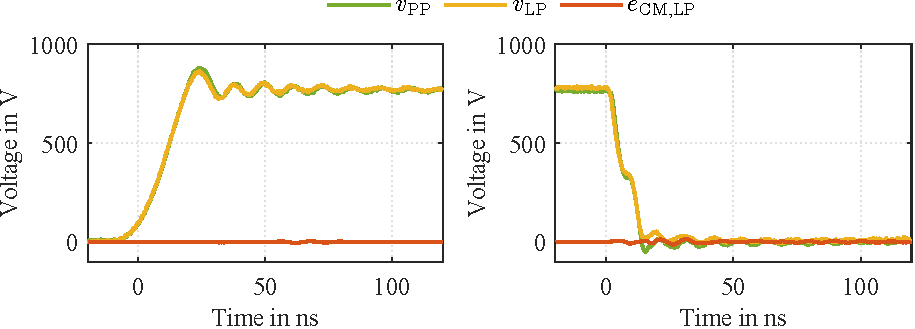
\includegraphics[scale=1]{figures/4_VoltageProbe/Voltage_DPT_LPvsPP_weCM_TD.pdf}
	\caption{Time-domain measurement results of PMTX05, at 800V, 30A room temperature, cross validation of passive probe and low-pass measurement to crosscheck inductive and capacitive coupling effects.}\label{fig:Voltage_DPT_LPvsPP_weCM_TD}
\end{figure}

The low-pass measurement again shows close agreement with the passive probe, indicating that the active probe does not introduce additional parasitic coupling paths that would materially distort the drain-source voltage waveform.
The remaining deviation is consistent with the limited large-signal settling behavior discussed previously and is most visible during the faster active-on transition, which exhibits a settling interval of approximately \SI{14}{ns}, compared with about \SI{32}{ns} during active-off switching.
The dedicated common-mode measurement furthermore shows that the residual common-mode error remains below \SI{4}{V} during active-off and below \SI{14}{V} during active-on, corresponding to less than \SI{1.8}{\percent} of the measured voltage.
These values confirm that common-mode feedthrough remains a secondary error source for the intended switching analysis.

Additionally, \fref{fig:Voltage_DPT_HPvsPP_weCM_TD} shows the time domain high-pass channel measurement with a differential and common-mode error measurement.
Here, also, only a small change is measured.

\begin{figure}[ht]
	\centering
	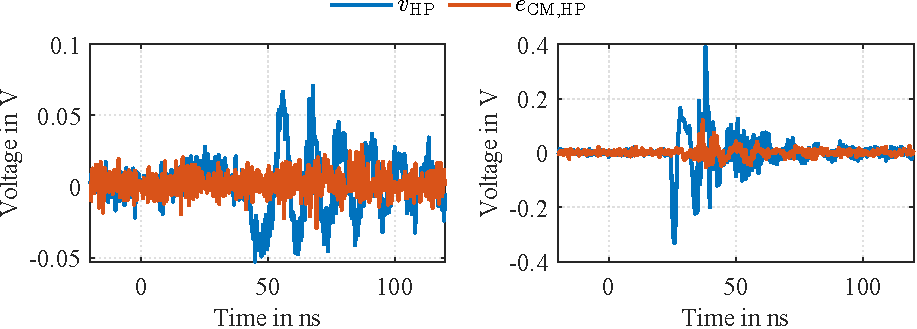
\includegraphics[scale=1]{figures/4_VoltageProbe/Voltage_DPT_HPvsPP_weCM_TD.pdf}
	\caption{Time-domain measurement results of PMTX05, at 800V, 30A room temperature, cross validation of passive probe and high-pass measurement to crosscheck inductive and capacitive coupling effects.}\label{fig:Voltage_DPT_HPvsPP_weCM_TD}
\end{figure}




\subsection{Noise Behavior}
The final step of this section is not a strict verification, but rather a characterization of the probe's noise behavior.
This analysis clarifies the probe limitations and provides context for interpreting subsequent measurement results.


Figure~\ref{fig:Diss_Voltage_NoiseContribution} shows the frequency-domain noise behavior for an acquisition length corresponding to the pulse chain duration used later (\SI{5}{ms}).
First, the high-pass channel was measured at the oscilloscope resolution used for subsequent signal measurements (Probe + HV Resolution).
Second, a noise measurement was performed at the same resolution with the probe disconnected (HV Resolution).
Third, the measurement was repeated with the probe connected and full ADC resolution, which reduces quantization noise (Probe + Full Resolution).
Finally, a measurement without the probe and with full ADC resolution was performed to determine the oscilloscope noise floor (Full Resolution).

\begin{figure}[hbt]
	\centering
	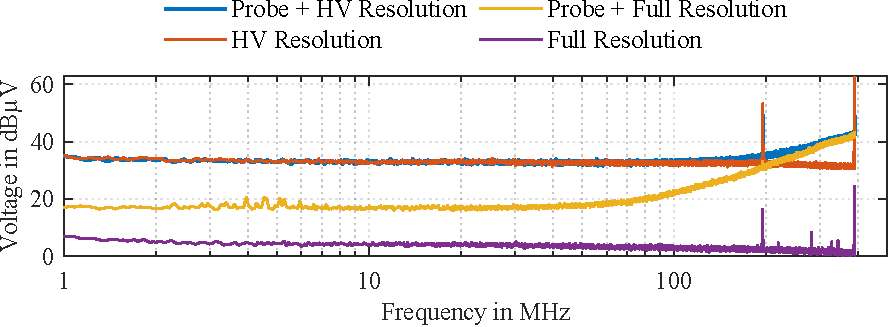
\includegraphics[scale=1]{figures/4_VoltageProbe/Diss_Voltage_NoiseContribution.pdf}
	\caption{Frequency domain measurement of the noise limiting effects of the EME voltage probe.}\label{fig:Diss_Voltage_NoiseContribution}
\end{figure}

Comparing the two no-probe measurements at different resolutions shows that quantization noise is the dominant contribution: the noise level decreases significantly from \SI{50}{dBµV} to \SI{22}{dBµV} when full ADC resolution is used.
With the probe connected, the intrinsic probe noise remains below the quantization-noise level of the HV-resolution measurement (\SI{33}{dBµV}) up to approximately \SI{100}{MHz}.
Above this frequency, the noise rises with the high-pass gain slope, which amplifies both signal and noise.
The crossover occurs at approximately \SI{200}{MHz}, beyond which intrinsic probe noise dominates over quantization noise.

Additionally, signal peaks can be seen at \SI{196}{MHz} and its harmonics.
This corresponds to the ADC interleaving frequency of the oscilloscope.
Interleaving is a technique used in oscilloscopes to increase the effective sampling frequency by operating multiple ADCs in parallel, each sampling at a fraction of the total rate.
Afterwards the signal is reconstructed by combining the outputs of the individual ADCs.
When not all ADCs are perfectly matched, this process can introduce spurious frequency components at the interleaving frequency and its harmonics, which is observed in the measurement.

\begin{figure}[hbt]
	\centering
	\import{./figures/4_VoltageProbe/}{Diss_Highpass_EME_NoiseSources_ESB.pdf_tex}
	\caption{Equivalent circuit diagram of the noise sources for the first high-pass amplification stage.}\label{fig:ESB_OP_noiseSources}
\end{figure}

To explain this behavior, an analytical noise calculation is performed for the second high-pass amplification stage.
Figure~\ref{fig:ESB_OP_noiseSources} shows the equivalent circuit of the noise sources in the high-pass amplifier, where \mi{Z}{g} is the series connection of the feedback capacitor and resistor.
Each resistor contributes Johnson–Nyquist thermal noise, while the capacitor itself does not generate thermal noise and only contributes through its equivalent series resistance (ESR).
The operational amplifier adds both input voltage noise and input current noise.

The relevant noise contributions are:
\begin{itemize}
	\item incoming noise from preceding stages,
	\item amplifier input voltage noise,
	\item resistor thermal noise,
	\item amplifier input current noise.
\end{itemize}

The resistor thermal noise is given by
\begin{equation}
	\mi{V}{n,th} = \sqrt{4\mi{k}{B}TR\Delta f}.
\end{equation}

The effective noise gain of the high-pass stage is
\begin{equation}
	 NG = 1 + \frac{\mi{R}{f}}{\mi{Z}{g}}.
\end{equation}

The total output noise can then be expressed as
\begin{equation}
	\mi{v}{0} = \sqrt{(\mi{v}{n,in} NG)^2 + (\mi{v}{n} NG)^2 + 2(\mi{i}{n} \mi{R}{f})^2 + 2\cdot4\mi{k}{B}T\mi{R}{f}\Delta f + 2\cdot4\mi{k}{B}T\mi{R}{g}\Delta f \left(\frac{\mi{R}{f}}{\mi{Z}{g}}\right)^2}.
\end{equation}

This formulation highlights that the amplifier noise is amplified by the noise gain, and that the noise response inherits the high-pass characteristic of the stage.

Figure~\ref{fig:Diss_Voltage_NoiseCalc} shows the calculated noise contributions using the datasheet values.
The dominant noise source at low frequency is the amplifier's input current noise, while at higher frequencies the input voltage noise becomes dominant.
Resistor thermal noise is negligible because the resistor values are only a few hundred \si{\ohm}.

The input noise of the previous stage follows the same trend, it is basically the total noise of the first high-pass amplifier mulitplied with the noise gain of the second stage. 
The second cut off at \SI{100}{MHz} is clearly visible where the noise changes from first to second order.


\begin{figure}[hbt]
	\centering
	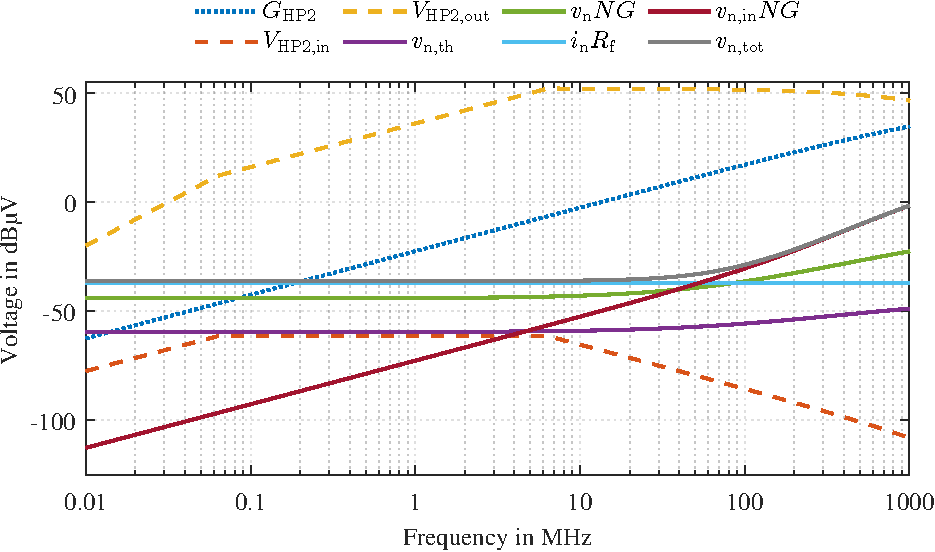
\includegraphics[scale=1]{figures/4_VoltageProbe/Diss_Voltage_Calc_Noise.pdf}
	\caption{Calculation of the noise sources for the first high-pass amplification stage.}\label{fig:Diss_Voltage_NoiseCalc}
\end{figure}





